\documentclass{standalone}
\usepackage{tikz}
\usetikzlibrary{patterns, positioning}

\begin{document}
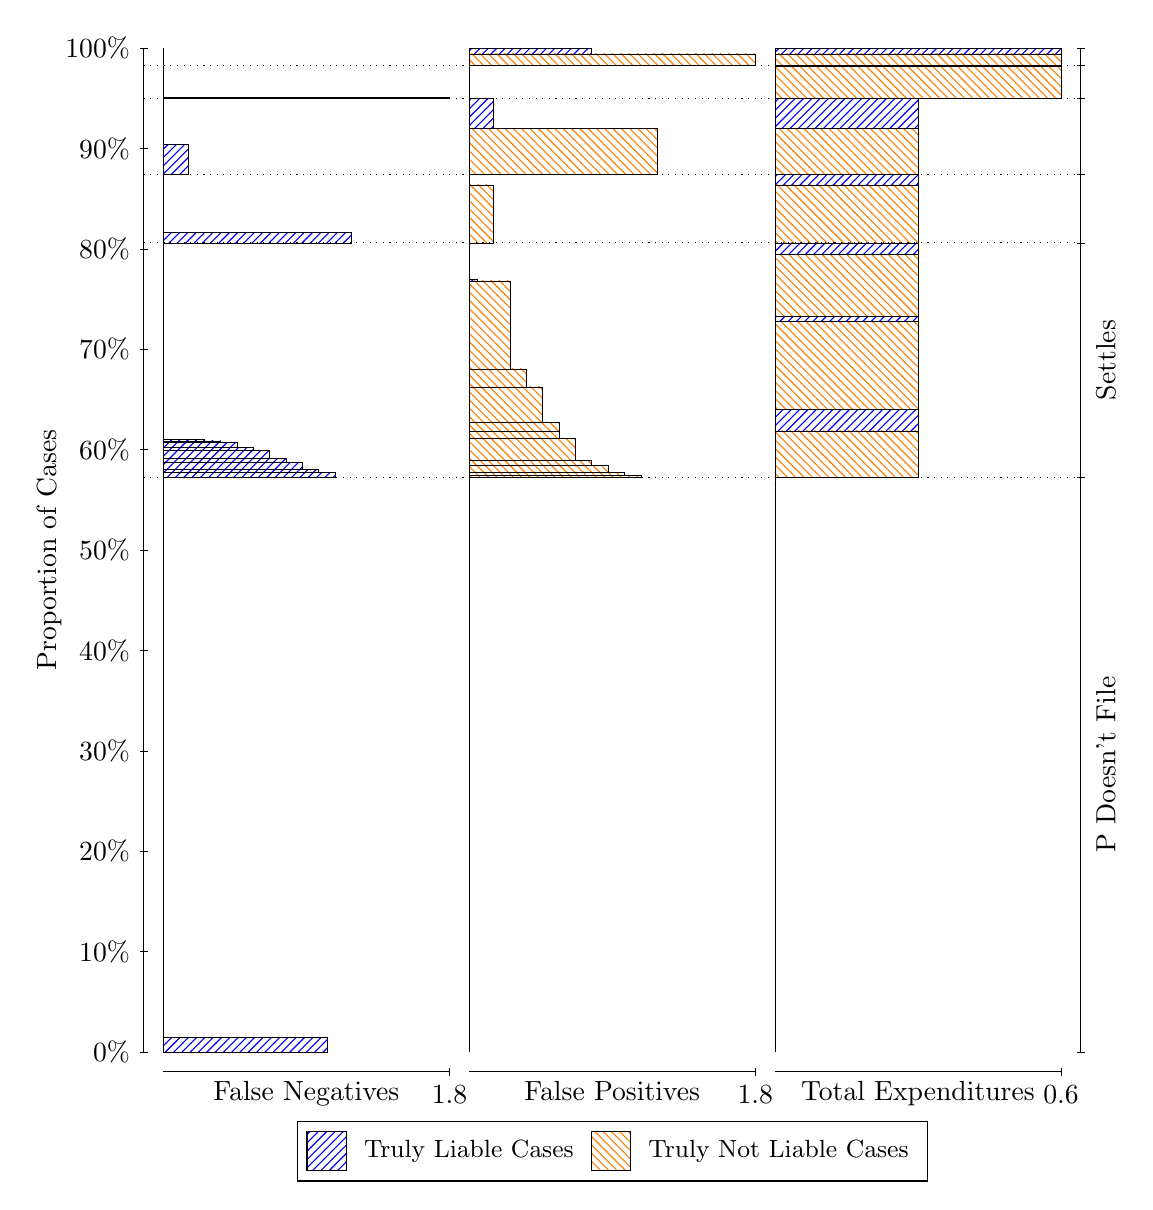
\begin{tikzpicture}
\draw[black, very thin] (1.5,1.75) -- (1.5,14.5);
\node[rotate=90, anchor=center] at (0.3, 8.125) {Proportion of Cases};
\draw[black, very thin] (1.45,1.75) -- (1.55,1.75);
\node[anchor=east] at (1.45, 1.75) {0\%};
\draw[black, very thin] (1.45,3.025) -- (1.55,3.025);
\node[anchor=east] at (1.45, 3.025) {10\%};
\draw[black, very thin] (1.45,4.3) -- (1.55,4.3);
\node[anchor=east] at (1.45, 4.3) {20\%};
\draw[black, very thin] (1.45,5.575) -- (1.55,5.575);
\node[anchor=east] at (1.45, 5.575) {30\%};
\draw[black, very thin] (1.45,6.85) -- (1.55,6.85);
\node[anchor=east] at (1.45, 6.85) {40\%};
\draw[black, very thin] (1.45,8.125) -- (1.55,8.125);
\node[anchor=east] at (1.45, 8.125) {50\%};
\draw[black, very thin] (1.45,9.4) -- (1.55,9.4);
\node[anchor=east] at (1.45, 9.4) {60\%};
\draw[black, very thin] (1.45,10.675) -- (1.55,10.675);
\node[anchor=east] at (1.45, 10.675) {70\%};
\draw[black, very thin] (1.45,11.95) -- (1.55,11.95);
\node[anchor=east] at (1.45, 11.95) {80\%};
\draw[black, very thin] (1.45,13.225) -- (1.55,13.225);
\node[anchor=east] at (1.45, 13.225) {90\%};
\draw[black, very thin] (1.45,14.5) -- (1.55,14.5);
\node[anchor=east] at (1.45, 14.5) {100\%};

\draw[black, very thin] (13.4,1.75) -- (13.4,14.5);
\draw[black, very thin] (13.35,1.75) -- (13.45,1.75);
\node[anchor=west] at (13.35, 1.75) {};
\draw[black, very thin] (13.35,9.0504) -- (13.45,9.0504);
\node[anchor=west] at (13.35, 9.0504) {};
\draw[black, very thin] (13.35,12.026) -- (13.45,12.026);
\node[anchor=west] at (13.35, 12.026) {};
\draw[black, very thin] (13.35,12.899) -- (13.45,12.899);
\node[anchor=west] at (13.35, 12.899) {};
\draw[black, very thin] (13.35,13.857) -- (13.45,13.857);
\node[anchor=west] at (13.35, 13.857) {};
\draw[black, very thin] (13.35,14.28) -- (13.45,14.28);
\node[anchor=west] at (13.35, 14.28) {};
\draw[black, very thin] (13.35,14.5) -- (13.45,14.5);
\node[anchor=west] at (13.35, 14.5) {};

\draw[black, very thin, pattern color=blue, pattern=north east lines] (1.75,1.75) rectangle (3.8262,1.9395);
\draw[black, very thin, pattern color=orange, pattern=north west lines] (1.75,1.9395) rectangle (1.75,9.0504);
\draw[black, very thin, pattern color=blue, pattern=north east lines] (1.75,9.0504) rectangle (3.93,9.1115);
\draw[black, very thin, pattern color=blue, pattern=north east lines] (1.75,9.1115) rectangle (3.7224,9.1459);
\draw[black, very thin, pattern color=blue, pattern=north east lines] (1.75,9.1459) rectangle (3.5148,9.2363);
\draw[black, very thin, pattern color=blue, pattern=north east lines] (1.75,9.2363) rectangle (3.3071,9.2846);
\draw[black, very thin, pattern color=blue, pattern=north east lines] (1.75,9.2846) rectangle (3.0995,9.3934);
\draw[black, very thin, pattern color=blue, pattern=north east lines] (1.75,9.3934) rectangle (2.8919,9.4281);
\draw[black, very thin, pattern color=blue, pattern=north east lines] (1.75,9.4281) rectangle (2.6843,9.4901);
\draw[black, very thin, pattern color=blue, pattern=north east lines] (1.75,9.4901) rectangle (2.4767,9.5117);
\draw[black, very thin, pattern color=blue, pattern=north east lines] (1.75,9.5117) rectangle (2.269,9.5336);
\draw[black, very thin, pattern color=orange, pattern=north west lines] (1.75,9.5336) rectangle (1.75,12.026);
\draw[black, very thin, pattern color=blue, pattern=north east lines] (1.75,12.026) rectangle (4.1376,12.163);
\draw[black, very thin, pattern color=orange, pattern=north west lines] (1.75,12.163) rectangle (1.75,12.899);
\draw[black, very thin, pattern color=blue, pattern=north east lines] (1.75,12.899) rectangle (2.0614,13.274);
\draw[black, very thin, pattern color=orange, pattern=north west lines] (1.75,13.274) rectangle (1.75,13.857);
\draw[black, very thin, pattern color=blue, pattern=north east lines] (1.75,13.857) rectangle (5.3833,13.873);
\draw[black, very thin, pattern color=orange, pattern=north west lines] (1.75,13.873) rectangle (1.75,14.28);
\draw[black, very thin, pattern color=orange, pattern=north west lines] (1.75,14.28) rectangle (1.75,14.425);
\draw[black, very thin, pattern color=blue, pattern=north east lines] (1.75,14.425) rectangle (1.75,14.5);
\draw[black, very thin, pattern color=orange, pattern=north west lines] (5.6333,1.75) rectangle (5.6333,8.8608);
\draw[black, very thin, pattern color=blue, pattern=north east lines] (5.6333,8.8608) rectangle (5.6333,9.0504);
\draw[black, very thin, pattern color=orange, pattern=north west lines] (5.6333,9.0504) rectangle (7.8133,9.0765);
\draw[black, very thin, pattern color=orange, pattern=north west lines] (5.6333,9.0765) rectangle (7.6057,9.1073);
\draw[black, very thin, pattern color=orange, pattern=north west lines] (5.6333,9.1073) rectangle (7.3981,9.1961);
\draw[black, very thin, pattern color=orange, pattern=north west lines] (5.6333,9.1961) rectangle (7.1905,9.2655);
\draw[black, very thin, pattern color=orange, pattern=north west lines] (5.6333,9.2655) rectangle (6.9829,9.5471);
\draw[black, very thin, pattern color=orange, pattern=north west lines] (5.6333,9.5471) rectangle (6.7752,9.638);
\draw[black, very thin, pattern color=orange, pattern=north west lines] (5.6333,9.638) rectangle (6.7752,9.7416);
\draw[black, very thin, pattern color=orange, pattern=north west lines] (5.6333,9.7416) rectangle (6.5676,10.196);
\draw[black, very thin, pattern color=orange, pattern=north west lines] (5.6333,10.196) rectangle (6.36,10.424);
\draw[black, very thin, pattern color=orange, pattern=north west lines] (5.6333,10.424) rectangle (6.1524,11.543);
\draw[black, very thin, pattern color=blue, pattern=north east lines] (5.6333,11.543) rectangle (5.7371,11.565);
\draw[black, very thin, pattern color=blue, pattern=north east lines] (5.6333,11.565) rectangle (5.6333,12.026);
\draw[black, very thin, pattern color=orange, pattern=north west lines] (5.6333,12.026) rectangle (5.9448,12.762);
\draw[black, very thin, pattern color=blue, pattern=north east lines] (5.6333,12.762) rectangle (5.6333,12.899);
\draw[black, very thin, pattern color=orange, pattern=north west lines] (5.6333,12.899) rectangle (8.021,13.482);
\draw[black, very thin, pattern color=blue, pattern=north east lines] (5.6333,13.482) rectangle (5.9448,13.857);
\draw[black, very thin, pattern color=orange, pattern=north west lines] (5.6333,13.857) rectangle (5.6333,14.263);
\draw[black, very thin, pattern color=blue, pattern=north east lines] (5.6333,14.263) rectangle (5.6333,14.28);
\draw[black, very thin, pattern color=orange, pattern=north west lines] (5.6333,14.28) rectangle (9.2667,14.425);
\draw[black, very thin, pattern color=blue, pattern=north east lines] (5.6333,14.425) rectangle (7.1905,14.5);
\draw[black, very thin, pattern color=orange, pattern=north west lines] (9.5167,1.75) rectangle (9.5167,8.8608);
\draw[black, very thin, pattern color=blue, pattern=north east lines] (9.5167,8.8608) rectangle (9.5167,9.0504);
\draw[black, very thin, pattern color=orange, pattern=north west lines] (9.5167,9.0504) rectangle (11.333,9.638);
\draw[black, very thin, pattern color=blue, pattern=north east lines] (9.5167,9.638) rectangle (11.333,9.9094);
\draw[black, very thin, pattern color=orange, pattern=north west lines] (9.5167,9.9094) rectangle (11.333,11.029);
\draw[black, very thin, pattern color=blue, pattern=north east lines] (9.5167,11.029) rectangle (11.333,11.09);
\draw[black, very thin, pattern color=orange, pattern=north west lines] (9.5167,11.09) rectangle (11.333,11.876);
\draw[black, very thin, pattern color=blue, pattern=north east lines] (9.5167,11.876) rectangle (11.333,12.026);
\draw[black, very thin, pattern color=orange, pattern=north west lines] (9.5167,12.026) rectangle (11.333,12.762);
\draw[black, very thin, pattern color=blue, pattern=north east lines] (9.5167,12.762) rectangle (11.333,12.899);
\draw[black, very thin, pattern color=orange, pattern=north west lines] (9.5167,12.899) rectangle (11.333,13.482);
\draw[black, very thin, pattern color=blue, pattern=north east lines] (9.5167,13.482) rectangle (11.333,13.857);
\draw[black, very thin, pattern color=orange, pattern=north west lines] (9.5167,13.857) rectangle (13.15,14.263);
\draw[black, very thin, pattern color=blue, pattern=north east lines] (9.5167,14.263) rectangle (13.15,14.28);
\draw[black, very thin, pattern color=orange, pattern=north west lines] (9.5167,14.28) rectangle (13.15,14.425);
\draw[black, very thin, pattern color=blue, pattern=north east lines] (9.5167,14.425) rectangle (13.15,14.5);
\draw[black, dotted] (1.5,9.0504) -- (13.4,9.0504);
\draw[black, dotted] (1.5,12.026) -- (13.4,12.026);
\draw[black, dotted] (1.5,12.899) -- (13.4,12.899);
\draw[black, dotted] (1.5,13.857) -- (13.4,13.857);
\draw[black, dotted] (1.5,14.28) -- (13.4,14.28);
\draw[black, very thin] (1.75,1.5) -- (5.3833,1.5);
\node[anchor=north] at (3.5667, 1.5) {False Negatives};
\draw[black, very thin] (5.3833,1.45) -- (5.3833,1.55);
\node[anchor=north] at (5.3833, 1.45) {1.8};

\draw[black, very thin] (5.6333,1.5) -- (9.2667,1.5);
\node[anchor=north] at (7.45, 1.5) {False Positives};
\draw[black, very thin] (9.2667,1.45) -- (9.2667,1.55);
\node[anchor=north] at (9.2667, 1.45) {1.8};

\draw[black, very thin] (9.5167,1.5) -- (13.15,1.5);
\node[anchor=north] at (11.333, 1.5) {Total Expenditures};
\draw[black, very thin] (13.15,1.45) -- (13.15,1.55);
\node[anchor=north] at (13.15, 1.45) {0.6};

\node[black, centered, rotate=90] at (13.72, 5.4002) {P Doesn't File};
\node[black, centered, rotate=90] at (13.72, 10.538) {Settles};





\draw (7.449999999999999,1.5) node[draw=none] (baseCoordinate) {};
\begin{scope}[align=center]
        \matrix[scale=0.5, draw=black, below=0.5cm of baseCoordinate, nodes={draw}, column sep=0.1cm]{
            \node[rectangle, draw, minimum width=0.5cm, minimum height=0.5cm, pattern=north east lines, pattern color=blue] {}; &
            \node[draw=none, font=\small] (B) {Truly Liable Cases}; &
            \node[rectangle, draw, minimum width=0.5cm, minimum height=0.5cm, pattern=north west lines, pattern color=orange] {}; &
            \node[draw=none, font=\small] (B) {Truly Not Liable Cases}; \\
            };
\end{scope}

\end{tikzpicture}
\end{document}